\title{Assignment 1: CS 763}
\author{
  Sai Charith \\ 160050083
  \and
  Sanchit Jain\\ 160050043  
  \and
  Mayank Singhal\\ 160050039 
}

\documentclass[a4paper]{article}
\usepackage{amsmath}

\usepackage{amsfonts,amssymb,amsthm}
\usepackage[margin=0.94in]{geometry}
\usepackage{graphicx}
\usepackage{subfigure}
\begin{document}
\maketitle
%\makebox[\linewidth]{\rule{\paperwidth}{0.4pt}}
%\noindent\rule{12cm}{0.4pt}
\hrulefill
\\ \\



\textbf{\newline Problem 2}
Motion model used is affine with translation, rotation and scale.


\begin{figure}[ht!]
\subfigure[x]{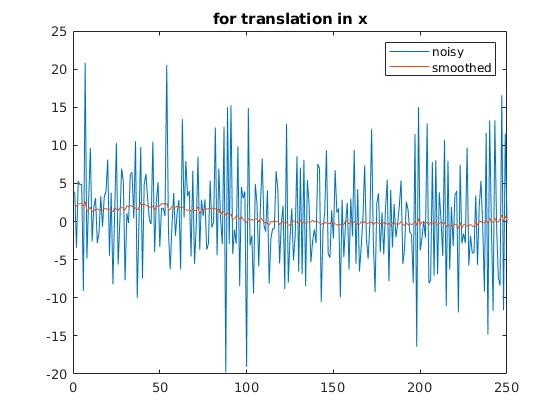
\includegraphics[width=0.5\textwidth]{Q2/output/cars_x.jpg}}
\hfill
\subfigure[y]{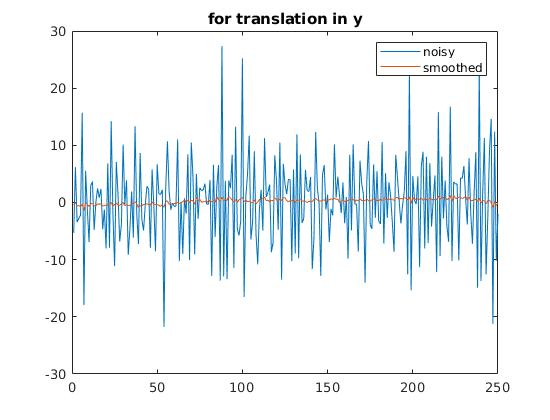
\includegraphics[width=0.5\textwidth]{Q2/output/cars_y.jpg}}
\subfigure[theta]{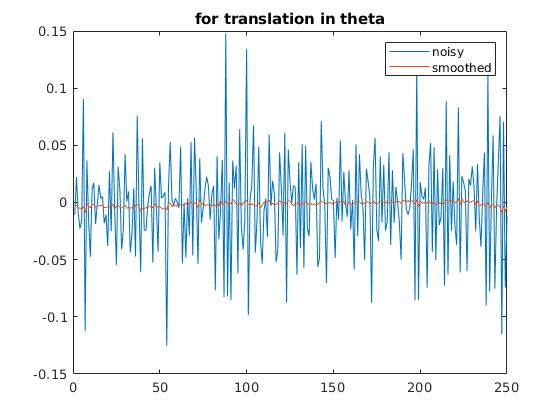
\includegraphics[width=0.5\textwidth]{Q2/output/cars_theta.jpg}}
\subfigure[scale]{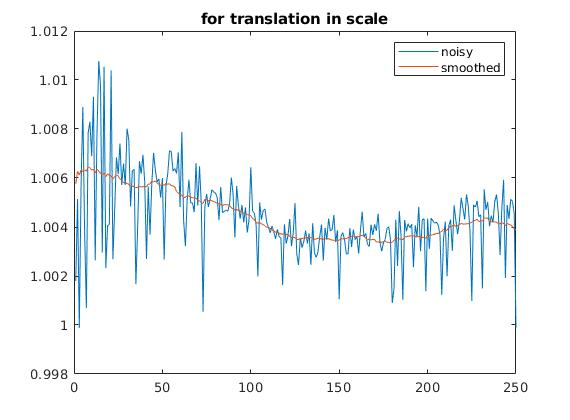
\includegraphics[width=0.5\textwidth]{Q2/output/cars_scale.jpg}}
\caption{Shaky car}
\end{figure}

\begin{figure}[ht!]
\subfigure[x]{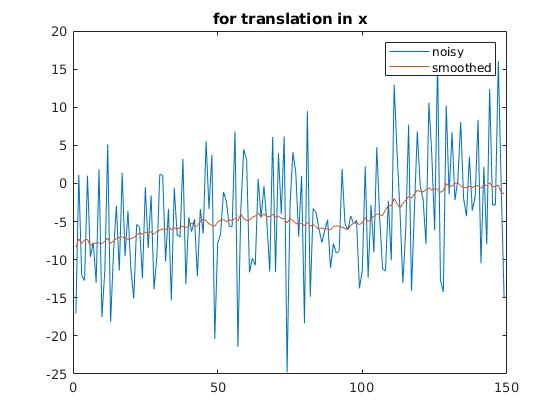
\includegraphics[width=0.5\textwidth]{Q2/output/bus_x.jpg}}
\hfill
\subfigure[y]{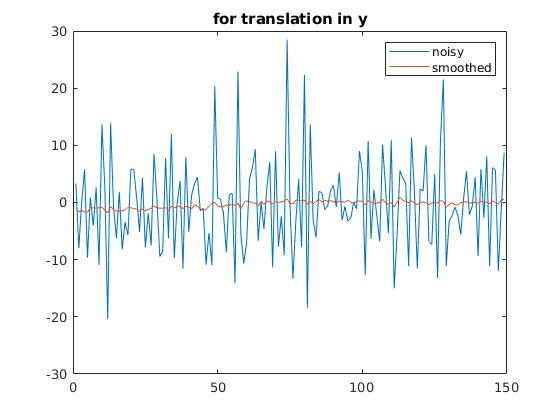
\includegraphics[width=0.5\textwidth]{Q2/output/bus_y.jpg}}
\subfigure[theta]{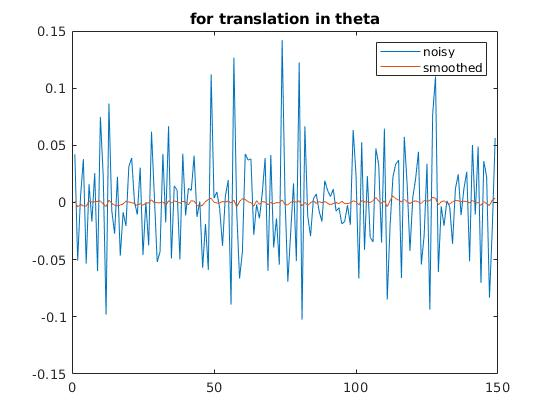
\includegraphics[width=0.5\textwidth]{Q2/output/bus_theta.jpg}}
\subfigure[scale]{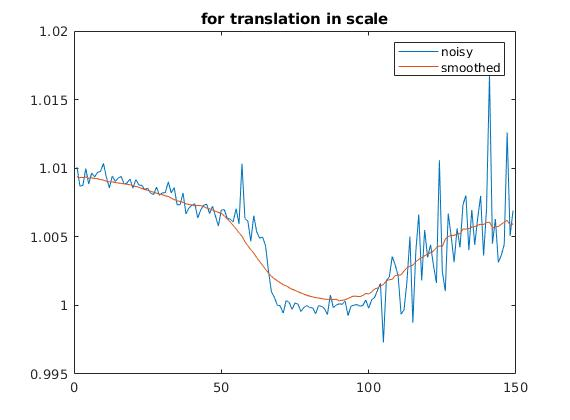
\includegraphics[width=0.5\textwidth]{Q2/output/bus_scale.jpg}}
\caption{Shaky bus}
\end{figure}



\end{document}
